\documentclass[10pt,a4paper,onecolumn]{report}
\usepackage[margin=0.5in]{geometry}
\usepackage[utf8]{inputenc}
\usepackage{amsmath}
\usepackage{amsfonts}
\usepackage{amssymb}
\usepackage{pdfpages}
\usepackage[comma,sort&compress]{natbib}

\usepackage{listings}
\bibliographystyle{h-physrev3}
\setcitestyle{numbers,square}
\usepackage{graphicx}
\graphicspath{figs} 
\begin{document}
\title{UnitedAtom and CoronaKMC user guide}

\maketitle 

\chapter{Introduction}
This document is designed to provide an overview of how to run the UnitedAtom and CoronaKMC packages for the prediction of nanoparticle (NP) to protein adsorption energies and the composition of the corona for an NP immersed in a particular environment. It is assumed that you have access to the publications describing the theory behind these tools and so this document will focus more on practical details about running the software packages.

Throughout, we use the convention that the substrate is a ``nanoparticle'' and the adsorbates are ``proteins'' to fit with the initial usage of UnitedAtom, where a ``protein'' is an assembly of ``amino acids'' (AA). In general, the protein can be any molecule which can be modelled as a set of component beads.

\section{Installation}
The most recent version of the code can be obtained using git from a repository stored on bitbucket:
\begin{lstlisting}
git clone https://bitbucket.org/softmattergroup/unitedatom.git
\end{lstlisting}

UnitedAtom is written in C++ with all source files stored in the src directory and can be compiled using the command
\begin{lstlisting}
make clean; make
\end{lstlisting}
which will require a C++ compiler and the Boost libraries to be installed.

The current version of CoronaKMC is implemented in Python 3 and is the CoronaKMC-P3.py script. An older version (CoronaKMC.py) is provided for Python 2.7 users but is no longer maintained and is lacking a significant amount of functionality compared to more recent versions. 
 
\section{High-level pipelines}
A frequent use case is the prediction of the corona for a simple nanoparticle (e.g. a sphere of a predefined material) in a medium consisting of proteins of known concentration. In this case, the provided PrepareKMCInput.py script is designed to automate the process and can be run using a command such as:

\begin{lstlisting}
python3 PrepareKMCInput.py -r [NPRadius] -z [ZETA] \\
-m [MATERIALNAME] -p [OUTPUTFOLDERNAME] -o [PROTEINSET] -t [CORONASIMULATIONTIME]
\end{lstlisting}
 where the first three options define the nanoparticle in question by radius (in nm), the excess surface potential of the NP beyond that included in the PMF (in mV) and the material from the list of predefined materials. The ``-p'' option defines the name of a folder in which to store the files generated. The ``-o'' option must be the path to a file containing a list of all biomolecules required to bepresent in the medium in the format,
 \begin{lstlisting}
 #comment lines start with a # and are ignored during parsing
 #all other lines are split by a comma into a protein name and a concentration in mol/L
protein1,1e-4
protein2,0.003
smallmolecule1,0.01
\end{lstlisting}
Each line in this file is required to have a matching structure stored in the allproteins folder, e.g. ``protein1.pdb'', ``protein2.pdb'', ``smallmolecule1.pdb''. The -t option defines how many seconds of simulated time to run the corona simulation for. Further options are available and can be found using 
\begin{lstlisting}
python3 PrepareKMCInput.py --help
\end{lstlisting}
which lists all the available commands and details about what they do. 
 
 
 
\chapter{UnitedAtom}
 \section{Introduction}
 In brief, UnitedAtom takes as input a set of potentials representing NP-AA interactions for a specific nanomaterial (e.g. anatase, amorphous carbon), a structure built from a set of AAs, and some variables defining a particular nanoparticle from the underlying nanomaterial (e.g. a 5 nm gold sphere with an extra applied surface potential of $+10$mV). The output is then a table of data representing the adsorption affinity of each orientation of the input structure relative to the surface of the NP, commonly plotted as a heatmap.
  Running UA is in principle straightforward. Store the protein/biomolecule structures of interest in a folder, make sure you have a set of PMFs and Hamaker constants describing the short range and long range AA-NP interactions respectively, edit the configuration file to select these, use the command
\begin{lstlisting}
./UnitedAtom --config-file=myconfigfile.config
\end{lstlisting}
to start UnitedAtom and then go wait a while (typically, up to a few minutes per protein per NP) until its done. 


\subsection{What's it actually doing?}
A run of UA works briefly as follows:

\begin{enumerate}
\item Read in the config file
\item Load in the protein structures
\item Assemble all NP radius-zeta combinations for the chosen material OR load in all target NPs
\item For each NP, build the total potential for each AA interacting with that NP.
\item For each protein, rotate to a specified orientation, sum over AA potentials to get the protein-NP potential, integrate over distance to get an adsorption energy. Repeat multiple times at slight perturbations of each orientation to produce an average.
\item When orientation averaging is done, write results out to a file.
\item Repeat for next protein, then for next NP, until everything is done.

\end{enumerate}

 The orientation $\theta,\phi$ is defined such that the input co-ordinates are rotated by an angle of $-\phi$ around the z-axis, followed by a rotation of $\pi - \theta$ around the y axis. Note that because 3D rotations are non-commutative, you do not get the same results if you apply these in the opposite order and, moreover, the rotation around $z$ still has an effect even for a spherical NP because it alters which residues are moved by the second rotation step.  For cylinders and NP-complexes, a final rotation of $\omega$ is applied around the z axis after the $\theta$ rotation. This rotation is currently stored in the filename rather than the table of output for backwards compatability with post-processing scripts. This step is redundant for spherical NPs and is omitted for these. 

\section{Theory}
The theory is covered in many other places, so here is just a quick overview. The basic, one-NP version of UA constructs a potential for each AA bead species $S$
\begin{equation}
U_S(r) =   U_{surf}(S,r) + U_{el}(S,r) +  U_H(S,r)
\end{equation} 
 where $r$ is the distance between the centre of the NP and the centre of the bead, $U_{surf}$ is a short-range potential, $U_{el}$ is an electrostatic potential, and  $U_H$ is a Hamaker-like potential. $U_{surf}$ is a tabulated potential extracted from metadynamics simulations to include the very close range repulsion, some electrostatic terms, solvent effects, mid-range vdW attraction, etc. A correction factor is applied to map these from the tabulated form generally computed for a plane to an NP of finite radius of curvature. The electrostatic term is evaluated in the Debye-Huckel approximation and has simple forms for the spherical,
 \begin{equation}
 U_el = ...
 \end{equation}
  cylindrical,
 \begin{equation}
 U_{el} = ...
 \end{equation}
and planar
  \begin{equation}
 U_{el} = ...
 \end{equation}

 cases. Finite cubes are evaluated using an expansion in spherical harmonics but are generally very well approximated by the planar expression, especially if the cube is large compared to the Debye length. 

 
 
  The Hamaker-like potential is an integral of the $1/r^6$ vdW potential over the volumes of the NP and bead, neglecting elements with a distance less than the exclusion distance $r_e$
 \begin{equation}
 U_H(S,r) \propto \int \int \frac{1}{r'^6} \Theta_H( r' - r_e)dV_{NP} dV_{AA}
 \end{equation}
 where $r'$ is the distance between two elements $dV_{NP}, dV_{AA}$ and $\Theta_H$ is the Heaviside theta function which is zero for $r_e > r'$. This integral has a complex analytical solution for spherical NPs which is implemented into UA, and can be solved numerically for cylinders (also implemented). The result is a smooth function (see Figure \ref{fig:hamaker-exclusion}) which avoids introducing a discontinuity into the potential which would be caused if this potential was only switched on if the bead centre is at a certain distance from the NP.
 
 
\begin{figure} \label{fig:hamaker-exclusion}
    \centering
    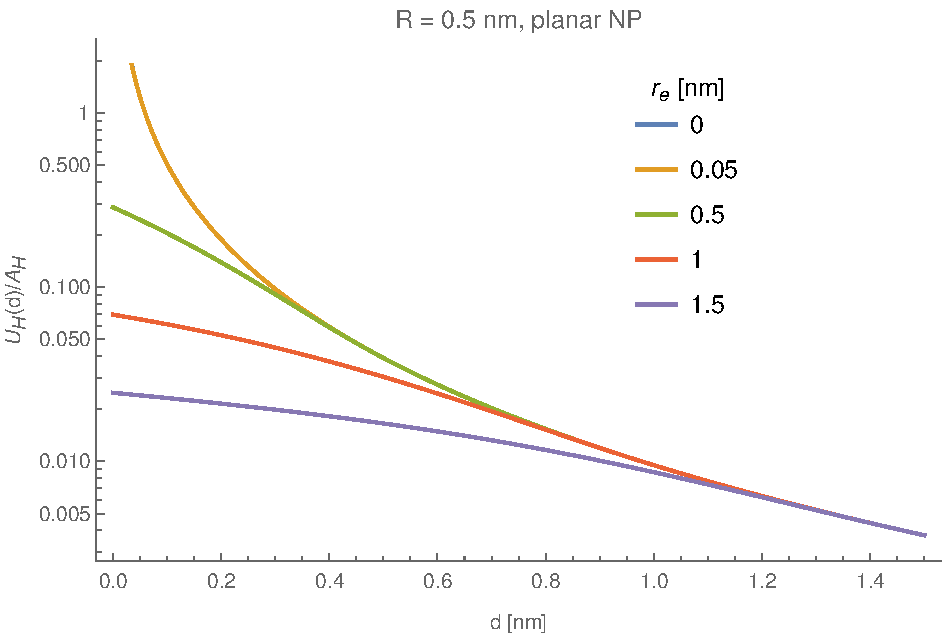
\includegraphics[width=0.6\textwidth]{figures/hamaker_magnitude_perresidue.pdf}
    \caption{Plots of the Hamaker-like potential used in UnitedAtom for an infinite planar NP and a residue of radius $0.5$ nm with surface-surface distance $d$, shown for multiple values of the exclusion distance $r_e$.}
\end{figure}
 
 
 
 
 
For a given protein consisting of a set of beads $j$ with species $S_j$ and NP-AA distances $r_j$, the total NP-protein potential is given by summation,
\begin{equation}
U_{AA-NP}(r_s)
\end{equation}
 where $r_s$ is a measure of the NP-protein distance, generally the closest approach or COM. 
 
 
 
\section{The configuration file}
 
\subsection{A standard file} 
 
 
Below is a standard UA configuration file, suitale for running a basic calculation of all structures in the all\_proteins folder for Anatase NPs of all combinaions given by the ``outer product'' of the nanoparticle-radius and zeta-potential lists, in this case: 5nm at -0.001V, 5 nm at 0 V, 5nm at 0.001 V, 10nm at -0.001V, 10nm at 0 V, 10 nm at 0.001 V. 

\begin{lstlisting}
#Autogenerated UA Config file, modified to show extra features
output-directory = UAOutput
pdb-target = all_proteins
nanoparticle-radius = [5.0, 10.0]
np-type = 1
pmf-directory = surface/TiO2-ana-101
hamaker-file = hamaker/TiO2_Anatase.dat
enable-surface 
enable-core 
enable-electrostatic 
simulation-steps = 2000 
potential-cutoff=5.0 
potential-size = 1000 
angle-delta = 5.0 
bjerum-length=0.716 
debye-length=0.785 
temperature = 300.0
zeta-potential = [-0.001, 0, 0.001] 
amino-acids         = [ ALA, ARG, ASN, ASP, CYS, GLN, GLU, GLY, HIS, ILE, LEU, LYS, MET, PHE, PRO, SER, THR, TRP, TYR, VAL] 
amino-acid-charges  = [ 0.0, 1.0, 0.0, -1.0, 0.0, 0.0, -1.0, 0.0, 0.5, 0.0, 0.0, 1.0, 0.0, 0.0, 0.0, 0.0, 0.0, 0.0, 0.0, 0.0] 
amino-acid-radii    = [ 0.323, 0.429, 0.362, 0.356, 0.352, 0.386, 0.376, 0.285, 0.302, 0.401, 0.401, 0.405, 0.402, 0.421, 0.362, 0.328, 0.357, 0.449, 0.425, 0.377] 
\end{lstlisting}
In order:
\begin{itemize}
\item output-directory : Folder in which to save output files. 
\item pdb-target : Parent directory for pdb structures, all files with a .pdb file extension  in all subfolders of this directory are used as input. Or a single file can be specified. 
\item nanoparticle-radius : A single value or list of NP radii in nm to scan over.
\item np-type : Shape ID. 1 = sphere, 2 = cylinder (with planar PMFs), 3 = cube (with planar PMFs), 4 = tube/hollow cylinder (with cylindrical PMFs), 5 = dense cylinder (with cylindrical PMFs). This selects the integration method, Hamaker function and PMF scaling.
\item pmf-directory : Folder containing XXX.dat files for each AA bead.
\item hamaker-file : File containing Hamaker data for all beads for that surface.
\item enable-surface : Switch to include short-range potential (should be always on)
\item enable-core : Switch to include Hamaker potential (should be always on, use Hamaker Null.dat to disable)
\item enable-electrostatic : Switch to include electrostatic potential (should be always on, use zeta = 0 to disable instead)
\item simulation-steps, potential-cutoff, potential-size,angle-delta : Leave as default values. These are largely overwritten internally.
\item bjerum-length : in principle the Bjerrum length, in practice does nothing except if a very specific other option is enabled and it almost surely won't be. The standard UA electrostatic expression does not include the Bjerrum length. If you are writing/reading anything and the electrostatic expression uses the Bjerrum length, you/the author are mistaken. 
\item debye-length : the Debye length for electostatic interactions. This actually is used. 
\item temperature : the ``temperature'', used as a scaling factor to change interactions. Experimental, best left at 300K unless you're sure you know what you're doing. 
\item zeta-potential : Single number or list, values for the ``zeta'' potential in V (so usually quite small, as -50 to +50 mV is the normal range). Note that internally this is actually the potential at the surface of the NP, the zeta potential will be smaller. 
\end{itemize}


The last three lists define the AA (or other small molecule) beads present. The first list defines each bead as a three-character ID code - note that longer codes will have undefined behaviour, likely leading to errors. The next two lists contain the charge and radius associated with each bead tag as in the above example, e.g. ALA is defined with a charge of 0.0 and radius 0.323, ARG with charge +1.0 and radius 0.429, etc.  Additionaly, the Hamaker file must contain an entry for each bead tag, and the PMF folder must contain a TAG.dat file for each bead, e.g. ALA.dat, ASP.dat.  

\subsection{Extra options}
The above general-purpose configuration file should be fine for most cases, but in certain circumstances some extra options may be needed. It is recommended that you check Config.h to see all available options, but here are some extra switches which can be enabled:

\begin{itemize}
\item pmf-cutoff : Set the Lennard-Jones cutoff used in the calculation of the short-range potential. This is assumed to be 1 nm by default, but if you used CHARMM for the calculation of PMFs it should be set to 1.2 nm. Note that this is the LJ cutoff and not the maximum distance recorded in the PMF. 
\item calculate-mfpt : Use mean-first-passage-time theory to estimate escape rates for the exact potential. This is very slow and generally unused.
\item np-target : This will be discussed more later. It overwrites the automatic generation of NPs and allows for multi-material or multi-bead NPs to be used. 
\item pmf-prefix : String used to differentiate between different surface potentials for the same bead as in "prefix-XXX.dat". Exists only for historical reasons. 
\item imaginary-radius : Used in testing of hollow NPs, can be ignored.
\item bounding-radius : Used primarily for multicomponent NPs, sets the radius at which the NP is taken to be solid and infinitely repulsive. Might be useful to edit if you're doing weird things and the auto-generated radius isn't working.
\item overlap-penalty : Value in kbT to penalise configurations in which a protein-bead overlaps an NP-bead. Used to mitigate problems with the multicomponent model by enforcing some anisotropy.
\item overlap-radiusfactor : Number $> 0$ , Used to resize AA beads for determining overlap with multicomponent models. Just leave it at 1 unless you have a really good reason not to. 
\item recalculate-zp : If non-zero, automatically adjust input zeta potentials to take into account the size of the NP and solution conditions, assuming that the input ZP corresponds to bjerrum length = 1 nm, debye length = 1nm, NP radius = 1nm. This is the only time the Bjerrum length matters and in practice you should just set the zeta potentials to whatever they actually are and not enable this option. 
\item save-potentials : If nonzero saves out the protein-NP potentials. Note that AA-NP potentials are automatically saved out to the pot-dat folder if this exists regardless of this option.
\item disorder-stategy : Enables extra options for dealing with disordered residues (those with b-factors between disorder-minbound and disorder-maxbound defined on the next two lines). If disorder-strategy = 0, these are treated as normal residues. If disorder-strategy = 1, these residues are moved to the centre of the protein.  disorder-strategy = 2 disables these residues entirely. These are most useful for dealing with AlphaFold structures with unphysical loops. 
\item disorder-minbound
\item disorder-maxbound
\end{itemize}


\section{Input data - Hamaker files}
The Hamaker file for a given material has the following format,
\begin{lstlisting}
#Name  kT        Joules        kJ/mol    
ALA    6.933     2.872E-20     17.332    
ARG    8.348     3.458E-20     20.869    
ASN    8.995     3.726E-20     22.487    
ASP    9.209     3.814E-20     23.022    
\end{lstlisting}
where the first column contains the three-letter tag associated with a given AA bead and the remaining columns are the NP-Water-AA Hamaker constant. These files are read by HamakerConstants.h with columns 1--7 providing the tag and columns 8--17 the energy in kBT (T=300), with all other entries ignored (but kept for ease of interpretation).


\section{Input data - Surface potential/PMFs}
The surface potential defines the short-range interaction between the NP and the AAs and is, typically, a potential of mean force including solvent effects, although any tabulated potential with a short-range repulsion will suffice. All beads defined in the configuration file with name XXX must have a corresponding XXX.dat file in the relevant directory. These files are defined in Surface.h and must be either comma-separated in the form distance(nm),energy(kj/mol) or with the distance stored in the columns 1--8 and the energy in columns 9--20, again in nm and kJ/mol. Empty lines and those starting with a \# are ignored. If the surface potential does not match this formatting you will probably get inconsistent results or an error. Comma formatting is strongly recommended! 

Important: UnitedAtom internally assumes that the PMFs used for input are either an infinite plane or an infinite cylinder (of radius 0.75 nm, to be specific). These are then corrected to the actual NP radius. If you've created PMFs for a small repeat unit, then UA will not give meaningful results because it will be trying to apply a correction to something that's already been corrected. You can either manually de-correct your PMFs to map from single bead to the equivalent of a plane or use multicomponent UA (discussed later) to build a raspberry model of your NP made from the individual beads. 

\section{Input structures - PDB}
The biomolecule to be scanned over is defined using a structure in the pdb format. The input file is read and each line is scanned in turn as implemented in PDBFile.h, with scanning continuing until the end of file or the first ``ENDMDL'' line is reached. Briefly, if columns 1 -- 4 contain the text "ATOM" and columns 14--15 the text "CA" then a bead is added to the internal structure for that molecule, else, the line is discarded.  The bead is defined based on the following entries:
\begin{itemize}
\item Column 18--20: bead ID tag
\item Column 31--38: x-coordinate (Angstrom)
\item Column 39--46: y-coordinate (Angstrom)
\item Column 47--54: z-coordinate (Angstrom)
\item Column 55--60: occupancy
\item Column 61--66: B-factor
\end{itemize}


Of these, the bead ID tag is used to select interaction potentials for that bead from the PMF folder and Hamaker file, and the x/y/z coordinates define where the bead is located. The occupancy gives an overall scaling factor for the potentials generated by that bead and is used such that disordered structures don't overcount beads and to allow for beads with multiple possible protonation states (e.g. histidine can be modelled as a HIE, HID, HIP bead triplet with occupancies summing to unity).  Thus, a single alanine bead can be represented by:

\begin{lstlisting}
ATOM      1  CA  ALA A   1       0.000   0.000   0.000  1.00  0.00
\end{lstlisting}
to make an ALA-type bead at 0,0,0 with occupancy 1, while histidine might be
\begin{lstlisting}
ATOM      1  CA  HIE A   1       0.000   0.000   0.000  0.62  0.00
ATOM      1  CA  HID A   1       0.000   0.000   0.000  0.16  0.00
ATOM      1  CA  HIP A   1       0.000   0.000   0.000  0.22  0.00
\end{lstlisting}
to produce a total of one residue but accounting for multiple possible charge states.


In general, these input structures can be taken directly from the PDB repository, from the AlphaFold prediction set or from I-TASSER output, or manually created. Two optional forms of pre-processing are suggested:

1) The protein can be rotated to ``canonical form'' using the ProteinSetRotate.py script, which rotates the protein such that the largest moment of intertia is associated with the z axis, second largest with the y axis, and the dipole moment along the x axis is negative. In practice, this generally ensures that a prolate protein is aligned with the z axis such that the $\theta = 90$ orientations are typically the most strongly adsorbing, creating a characteristic horizontal band in the heatmap plots. 

2) Propka processing: propka3 (must be installed separately!) is called for each protein in the set and used to estimate protonation state probabilities for all residues based on an input pH value. The structure is then updated so that all possible protonation states for each residue are included with that weighting in the occupancy field, and HIS is also modified to split into HID and HIE states. The result is a structure which smoothly interpolates between possible charge states at a given pH. Note that the structure itself is not denatured at all and so care must be used for pH changes significantly far from neutral. 

Note that both of the above are combined in the PreprocessProteins.py script.

For the purposes of UA, only lines with the ATOM and CA strings in the correct locations matter. It is strongly recommended that further metadata is included in the file where possible, since it's not a good idea to rely on filenames alone, especially when the same protein may have multiple structures.
 
\section{Output: the .uam file}
The main output of UA is a .uam file for each protein-NP pair, which has the following format:
\begin{lstlisting}
#phi theta EAds/kbT=300 Error(Eads)/kbT=300 min_surf-surf-dist/nm mfpt*DiffusionCoeff/nm^2 EAds/kJ/mol min_ProtSurf_NPCentre-dist/nm
0.0    0.0    -3.73681      0.01376       0.32033       -1.00000e+00  -9.32087      5.32033       
5.0    0.0    -3.73211      0.01528       0.31476       -1.00000e+00  -9.30914      5.31476       
10.0   0.0    -3.72567      0.01541       0.30752       -1.00000e+00  -9.29309      5.30752       
15.0   0.0    -3.72474      0.01652       0.30929       -1.00000e+00  -9.29075      5.30929       
20.0   0.0    -3.72432      0.02027       0.30895       -1.00000e+00  -9.28971      5.30895       
25.0   0.0    -3.72646      0.02086       0.31663       -1.00000e+00  -9.29504      5.31663       
\end{lstlisting}
Each row contains to one set of orientational samples for that protein-NP pair, divided into bins of $\theta,\phi$ values. These columns contain, in order:
\begin{itemize}
\item phi: Left-hand edge of the angular bin for $\phi$ values - note the average is generally $\phi + 2.5$
\item theta: Left-hand edge of the angular bin for $\theta$ values - note the average is generally $\theta + 2.5$
\item EAds/kbT=300: Average of the EAds value for that bin
\item Error(Eads): Standard deviation NOT STANDARD ERROR for that bin. Be very aware that this is an SD for error propagation! 
\item min\_surf-surf-dist : Distance between the closest bead centre and the surface of the NP. Yes, its bead centre and not surface-surface distance. This is due to how UA stores distances. 
\item mfpt*DiffusionCoeff : product of the estimated MFPT and an unknown diffusion coefficient - divide this value by your diffiusion coefficient to get the MFPT. This is usually set to -1 if the MFPT isn't calculated.
\item EAds/kJMol : Adsorption energy again, but in units kJ/mol to make converting between temperatures easier.
\item ProtSurf\_NPCentre dist: Distance beteen the centre of the NP and the closest AA centre - in other words, min-surf-surf + the radius of the NP.
\end{itemize}
 
 
\section{The RunUA.py interface, material sets and bead sets}
To avoid the need to manually generate a configuration file each time, it's strongly recommended to use the RunUA.py interface where possible. This script takes a few common options and builds an appropriate configuration file (including calculation of appropriate Debye lengths), then automatically calls UA to run the adsorption energy calculation. 

This script requires that both the material and set of AA beads are predefined (so that it can populate the configuration file with entries for both). The material dataset is  read from the ``MaterialSet.csv" and ``surface-pmfp/MaterialSetPMFP.csv'' to differentiate between manually constructed materials and the automatically generated set of materials generated using the PMFPredictor software package. In general, as an end-user only MaterialSet.csv will need editing. This file consists of a set of comma-separated lines of the form
\begin{lstlisting}
materialname,pmf-folder,hamaker-file,shape-ID
\end{lstlisting}
e.g.
\begin{lstlisting}
anatase100,surface/TiO2-ana-100,hamaker/TiO2_Anatase.dat,1
\end{lstlisting}
which registers a material with the name ``anatase100'', PMFs stored in ``surface/TiO2-ana-100'', a Hamaker file at ``hamaker/TiO2\_Anatase.dat'' and a shape ID of ``1'' (meaning the PMFs will be mapped from an infinite plane to a sphere).  Valid shape IDs are:
1 = plane-to-sphere
2 = plane-to-cylinder
3 = plane-to-cube
4 = 1.5 nm diameter cylinder to tube
5 = 1.5 nm diameter cylinder to cylinder
where ``tubes'' are hollow and ``cylinders'' are solid. 

The RunUA.py interface searches this dataset for a material with the name in the first column, then assigns Hamaker and PMF directories based on the remaining entries for this material. This script also automatically populates the amino-acids, amino-acid-charges, amino-acid-radii entries based on the chosen bead configuration, by default, ``beadsets/StandardAABeadSet.csv'', which looks like this:
\begin{lstlisting}
#List of beads to include in UA autogenerated config files, providing the three-letter code, charge and radius to write to config files.
#BeadID,Charge[e],Radius[nm]
ALA,0.0,0.323
ARG,1.0,0.429
ASN,0.0,0.362
ASP,-1.0,0.356
CYS,0.0,0.352
GLN,0.0,0.386
\end{lstlisting}

 Other files can be chosen to more easily vary bead parameters - this is useful if you have some beads defined only for certain surfaces or disagree with the radii assigned.


\section{Extending UA}
The golden rule: document everything you add! For beads include a SMILES code, for surfaces ideally provide a link to the input structure and details about metadynamics settings. Storage is cheap and metadata is invaluable, especially when it comes to trying to mix results from multiple groups.

\subsection{New materials}
Computing PMFs and Hamaker constants for a brand-new material is outside the scope of this guide, so here we simply assume you have a set of short-range potentials, plus Hamaker constants for this material with each of the 20 AAs (or a willingness to use Null.dat for these Hamakers). Make a folder for your material in the surface folder with a short but descriptive name, e.g. ``Au-100-FCC'' to denote gold, miller index 100, FCC crystal structure. Place all the computed PMFs in this folder with names ALA.dat, ARG.dat etc (one per bead). Add a file with the computed Hamaker constants and ideally the same or at least a similar name. For bonus points, update MaterialSets.csv so the material works with the wrapper scripts and also put a readme file in the folder describing what exactly the material represents, what forcefield was used, metadynamics settings, the solvent/pH/ionic strength, definition used for SSD, and convention used for amino acids (full vs side chain, convention for glycine and proline, histidine variants, any charge variants, etc). 

\subsection{New adsorbate beads}
UA will throw an exception if it tries to load a bead for a material without that bead defined, but otherwise as long as you have the XXX.dat file in the surface folder and an entry in the Hamaker file for a material, this should go ok and you should be able to include new beads just by including these in the configuration file with their name, radius and charge. Remember to only use three letters for the ID tag and to make this match what you use in the PDB input file. To save headaches, try to avoid starting the tag with an X (Y is probably also a bad idea) and make sure you remember what code is what bead. It's probably a good idea to make a .pdb file using a template similar to the one shown in Section \ref{section:pmfp} as this provides a record of the chosen tag, SMILES code, full molecule name and gives you something you can immediately use to test the molecule in UA. 

\section{Multicomponent mode}
For a reasonably isotropic NP the above operation mode suffices, with core-shell NPs approximated via custom materials with one set of surface potentials and a different set of Hamaker potentials. In general, though, a more flexible approach may be needed. This is achieved through adding an extra line to the configuration file:
\begin{lstlisting}
np-target mynpfolder
\end{lstlisting}
If this line exists, UA no longer automatically generates NPs of the specified material/radius/shape. Instead, it reads in structures from this folder with each file corresponding to an NP-complex: a structure built from composite NP beads, analogously to how a protein is built from AA beads. This structure is constructed using NPFile.h which expects input of the form:

i.e. a comma separated string for each NP component, with every component on a new line. The columns are taken to be:
\begin{itemize}
\item x : x-coord of centre of NP component in nm
\item y : y-coord of centre of NP component in nm
\item z : z-coord of centre of NP component in nm
\item R : Radius of NP component
\item Zeta: electrostatic surface potential for the component (probably mV)
\item Core scale: prefactor applied to Hamaker potentials
\item Surface factor: prefactor applied to surface potentials
\item Shape: Shape ID. Shapes other than spheres are not very well tested and note that cylinders are always aligned to the x-axis.
\item Hamaker file: Path to the Hamaker file for that component
\item Surface set: Path to the directory of surface potentials
\item PMF cutoff: LJ cutoff for this component (to allow combining multiple methodologies)
\item Correction type: Manually change the surface correction applied to the surface potentials for this bead. This can probably be set to the same as the shape, except for small beads such as in polymer chains where it should be set to 0 because these don't need to be corrected as one bead = one molecule.
\end{itemize}


As an example:
\begin{lstlisting}
#x,y,z,R,zeta,corescale,surfacescale,shape,Hamaker,PMFSet,PMFCutoff,Correction
0,0,0,5.0,0,1,0,1,hamaker/Metal.dat,surface/Au/FCC/100/sca,1.2,1
1.085,4.159,2.554,0.5249,0,0,1,1,hamaker/PseudoPEG.dat,surface/PEG,1.2,0
1.137,4.536,2.702,0.525,0,0,1,1,hamaker/PseudoPEG.dat,surface/PEG,1.2,0
1.229,4.674,3.077,0.525,0,0,1,1,hamaker/PseudoPEG.dat,surface/PEG,1.2,0
1.028,4.944,3.286,0.525,0,0,1,1,hamaker/PseudoPEG.dat,surface/PEG,1.2,0
1.249,5.279,3.389,0.525,0,0,1,1,hamaker/PseudoPEG.dat,surface/PEG,1.2,0
\end{lstlisting}
will produce a 5nm gold NP decorated with a few PEG beads. Note the PMF cutoff is set to 1.2 nm because these potentials were computed using CHARMM and the PEGs use a correction type 0. The Hamaker terms for these beads can generally be set to 0, given their small size. 




The scaling factors can be arbitrary real values, with a typical use being the construction of a hollow NP by subtracting a small sphere from a large sphere, or a diffuse region with lower density. For example:
\begin{lstlisting}
#x,y,z,R,zeta,corescale,surfacescale,shape,Hamaker,PMFSet,PMFCutoff,Correction
0,0,0,5.0,0,1,1,1,hamaker/TiO2_Anatase.dat,surface/anatase-101,1.0,1
0,0,0,5.0,0,-1,-1,1,hamaker/Metal.dat,surface/Au/FCC/100/sca,1.2,1
0,0,0,6.0,0,1,1,1,hamaker/Metal.dat,surface/Au/FCC/100/sca,1.2,1
\end{lstlisting}
can be used to produce a 5nm anatase NP core with a 1nm coating of gold (i.e., a 6nm gold particle with scaling factors $+1$ and a 5nm gold particle with scaling factors $-1$. 


Complexes can be built using the GenerateNP.py script or other such tools, or through manual construction (not recommended, unless you have a lot of spare time). 

Caveats:

1) The surface of a complex NP is not well defined. Interpret binding energies with caution and try varying the bounding radius. 

2) In the default mode, the potentials are generated for single bead AAs at the north pole of the NP-complex and summation is done over this . This means that if there is a large enough gap for a single bead to sneak through, the entire protein will behave as if it can sneak into this space and dramatically overestimate the achievable binding energy. A hard-sphere repulsion can be switched on to reduce this effect.

Polymeric NPs (those for which the PMFs represent a small repeat unit rather than an entire slab) can be built using a raspberry model, check GenerateNP.py for examples, or as beads decorating the surface of a homogenous inner bead. For reasons of speed it's best to replace small inner beads by larger ones if you can, especially if they're at a distance of $> 1$ nm from the surface of the NP (and so only interact through the Hamaker potential) - summation of the potentials over all beads in an NP can be very slow, especially for larger radii. 


\section{PMFP} \label{section:pmfp}
If you've looked at the material sets (or read this guide) you might have noticed some files are tagged with ``pmfp'' or ``PMFP''. This refers to surface and Hamaker data predicted using the PMFPredictor repository, which uses machine learning methods to significantly increase the amount of materials and small molecules available for input to UA. A script in that repository produces bindings for UA to make use of the predictions, but as they are less rigorously tested and to distinguish them from metadynamics results they are assigned a different namespace. In brief, the PMFP datasets include a ``-pmfp'' tag in material names where appropriate. The generated beads are assigned an auto-generated 3 letter code starting with an X (unless they correspond to a standard bead, in which they use the same code). This results in a folder called ``hamaker-pmfp'' containing Hamaker files, ``surface-pmfp'' containing subdirectories with individual surfaces, a folder ``pmfp-beadsetdef'' containing a bead definition file ``PMFP-BeadSet.csv'' (three-letter code, radius, charge) and ``PMFP-BeadNames.txt'' which contains a lookup table for three-letter codes to the full name used in PMFPredictor. A folder ``pmfp-singlebead-pdbs'' is also supplied containing example PDBs for all the small molecules produced using PMFP, e.g.:
\begin{lstlisting}
HEADER CAFF-AC                                 23-Mar-23    XX4D
TITLE   CAFF-AC to bead X4D
REMARK SMILES: Cn1cnc2n(C)c(=O)n(C)c(=O)c12
REMARK Generated: 2023-03-23 10:03:05
ATOM      1  CA  X4D A   1       0.000   0.000   0.000  1.00  0.00
END
\end{lstlisting}
which may be used to generate binding energies for small molecules and contains sufficient metadata to identify the molecule used. 


\section{Source files}
In this section, the individual source files are discussed in more detail - if you need to modify UA or want to be sure how exactly something works, this is the place to start.

Parsers:
\begin{itemize}
\item CommandLineParser.h - read command line options
\item ConfigFileReader.h - read config files
\item Config.h - process config files
\item HamakerConstants.h - read Hamaker files
\item StringFormat.h - string helper functions
\item PDBFile.h - read PDB files
\item TargetList.h - find PDB files
\item NPFile.h - read NP input files
\item NPTargetList.h - find NP files

\end{itemize} 

Potentials:
\begin{itemize}
\item CubeESPotential.h - define the DH-like potential for cubes
\item CubePotential.h - define the Hamaker-like potential for cubes (centre of planar face)
\item CylinderPotential.h - define the Hamaker-like potential for infinite cylinders
\item TubePotential.h - define the Hamaker-like potential for infinite hollow cylinders
\item Surface.h - read PMFs and correct to target NP
\item Potentials.h - Combine all the potentials, build tables for each AA on the given NP, summing over NPs as needed. 
\end{itemize}

The main core of the program is contained in main.cpp, which handles the overall integration of potentials and orientational sampling. There are some inconsistencies in variable names, in particular: cutoff may mean either an LJ cutoff or the final point saved for a potential and ``SSD'' may mean surface-surface distance or surface-center distance depending on context. An attempt to standardise or at least comment on these has been made. 

\section{Post-processing and extra tools}
UnitedAtom output by itself typically requires some further processing to make it useful, since the raw data tends to be too much to directly analyse.

Note: in all that follows, be very careful to remember that the UA file format stores LEFT HAND EDGES for angles in units degrees. You therefore need to shift and convert to degrees, e.g.
\begin{lstlisting}
theta += 2.5
theta = theta*pi/180.0
\end{lstlisting}
early on or use
\begin{lstlisting}
sin((theta+2.5)*pi/180.0)
\end{lstlisting}
in all appropriate places.

A good first step is plotting a heatmap from the tables of binding energies. This can be done using the script in ``tools/plotmap'' or by importing the data into e.g. Mathematica and plotting contour plots (this can be better if you want a more smooth plot due to how tools/plotmap stores data, be aware that you can't just smooth it out using a Gaussian blur)

The next most common form of post-processing tends to be the evaluation of average adsorption energies as some form of weighted average,
\begin{equation}
\langle E \rangle = \frac{ \sum_i w_i E_i}{\sum_i w_i}
\end{equation}

where $w_i$ has two common forms. For the ``simple average'', $w_i = \sin \theta$ while for the Boltzmann average, $w_i = \sin \theta e^{-E_i/kbT}$. The former weights all states equally, e.g. for early corona formation, while the latter weights more strongly adsorbing states more strongly and is closer to the thermodynamic equilibrium for an NP with infinite binding locations such that competition between orientations can be neglected. 

In certain circumstances, it may be necessary to average across multiple .uam files. Be careful to identify what other weights need to be assigned and include them in $w_i$ if this is physically required to make a sensible average, and don't just assume that you can ``average the averages'' afterwards - this won't always give physically meaningful results


\section{Common issues and debugging tips}
UA is not foolproof, do not blindly accept your results as fact. Always test surfaces (especially new ones) against simple test molecules and conversely test molecules (especially AlphaFold/I-TASSER proteins) against the well-characterised surfaces to make sure these results are physically meaningful. In particular make sure you understand how orientations are defined with respect to the NP surface. It can be really useful to define simple dipole-like molecules with one strongly adsorbing end and one weakly adsorbing end as a simple test to make sure any post-processing script is giving sensible answers - for example, if you set the zeta potential to a large positive value (e.g. on the order volts) then a protein consisting of one LYS and one GLU should adsorb mostly strongly when GLU is on the surface.

A few rules of thumb:

\begin{itemize}
\item The most important factor by far is the number of residues directly in contact with the NP (distances $< 0.6 $ nm or so. 
\item The integration free energy is in practice essentially a soft minimum, especially for strongly binding proteins - remember that a difference of $1 k_BT$ in an exponential is a factor of $2.7$ in relative probabilities, so if there's a strongly binding configuration this typically outweights most other factors.
\item The short-range potential is typically the most important contribution, so you can usually get a feel for how strongly a protein will bind by looking at the most strongly binding PMFs and multiplying the depth of these by the number of protein-NP contacts. 
\item For typical electrostatic potentials of $\pm 50$ mV the electrostatic term typically only contributes a few $kbT$ at most per charged residue in contact with the NP. 
\item The long range (Hamaker) potential is generally the least significant. This is because it only takes into account parts of the NP/AA which are at a distance greater than $1$ nm from each other and by this point the $1/r^6$ potential has decayed to essentially zero. 
\end{itemize}


Some common problems:
\begin{itemize}
\item Binding energy is (almost) zero everywhere (0.06 seems typical) with (effectively) zero standard deviation. This means that the potential for your molecule is zero everywhere and the small residual is due to rounding issues in the numerical integration. Check the potentials and the PDB structures - if the columns aren't aligned correctly then the occupancy column may be reading as 0 for all residues.
\item Boost is complaining about file copying: this means you've renabled the code for saving config files (generally a good idea!) but you're using an older version of boost (generally a less good idea!) and one of their arbitrary breaking changes to do with how it handles overwriting files is breaking. Uncomment the alternative line or use the RunUA.py/PrepareKMCInput.py interfaces to save the config file automaticallly. 
\item The present version of UA won't automatically overwrite result files, so make sure your workflows save results to new folders as appropriate.
\end{itemize}


\chapter{CoronaKMC}
 \section{Introduction}
 CoronaKMC runs a hard-sphere simulation of the (usually reversible) adsorption of spherical particles onto a substrate based on input concentrations, particle sizes and per-site rate constants. The most typical use case is for the adsorption of proteins onto nanoparticle and this documentation is written with that in mind. 
 
 \section{How it works}
CoronaKMC-P3.py is the main script of interest here. It takes in a set of options and then performs the following
\begin{enumerate}
\item Prepare the list of all potential adsorbates
\item Begin the main loop
\item Use the Kinetic Monte Carlo algorithm to select events. Events can be adsorption of a protein from solution or desorption of a bound protein.
\item Continue until the preset time (simulation time, not wall time) is reached
\item Write out coverages, numbers, surface coordinates
\end{enumerate} 
 
 \section{Input}
CoronaKMC is controlled almost entirely through command-line arguments, unless you need to make very specific tweaks. These arguments can be viewed by running ``python3 CoronaKMC-P3.py --help'' and a summary of their meaning is given below:
 \begin{itemize}
 \item -r or --radius - the radius of the NP in nm. 
 \item -p or --proteins - The input file defining all adsorbates, see later
\item -s or --shape - shape of the NP,   1 = sphere, 2 = cylinder, 3 = plane, 4 = truncated sphere (i.e. a sphere but limited to only the upper part of the NP to save time)
\item -t or --time - Number of hours of simulated time (internal time, not wall time). Generally only a few seconds are needed, this is in hours for historical reasons.
\item --timedelta - Time step in seconds between showing updates, this will likely need some tweaking so you get updates reasonably frequently without being too quick to follow.
\item --demo - enables the demonstration mode (a live updating graph and corona figure)
\item -P or --projectname - name for the output folder used. 
\item -x or --npconc - concentration of NPs, leave zero for vanishing concentration. This is used to deplete proteins during simulation and so is appropriate for in vitro studies if the serum concentration is low. If proteins can be replenished from outside the NP concentration should be set to zero.
\item  -n or --numnp - number of NPs to run simultaneously, defaults to 1 and should be left at 1 unless you want to simulate protein depletion using the --npconc option (in which case it should be increased to reduce fluctuations). If you have npconc = 0 then just run multiple KMC runs at the same time instead for speed reasons.
\item  -D or --displace - activate the ``displacement mode'' if non-zero, where a protein can displace bound proteins if this is energetically favourable. 
\item -A or --accelerate - activate Dybeck style acceleration if set non-zero, with 1 giving the classic mode and 2 giving the mode with freezing of rate constants. This may need some tweaking to the code to give sensible results. 
\item -f or --fileid - optional string to append to output filenames to allow for multiple runs with similar configurations without overwriting each other (e.g. to get better averages).
\end{itemize}

Some optional ones are listed below - these tend to be for debugging or more specialised cases 
 
 \begin{itemize}
\item -l or --loadfile - load in a .kmc file from a previous run to precoat the NP in these proteins. Once these desorb they're lost forever. No sanity checks are made to make sure the NP between the two runs match!
\item -d or --diffuse - enable surface diffusion of bound proteins, currently only possible for spherical NPs. This is extremely slow and largely irrelevant. Activate only if needed.
\item -c or --coarse - this is mostly unneeded in the PrepareKMCInput.py pipeline but in effect allows for an orientational-averaging of all adsorbates to get an effective binding energy and area. The envisaged usage is that this lets you run a simulation of all orientations of a specific protein competing for binding and can back-calculate an effective binding energy and area which would produce the same number and surface coverage.
\item -m or --meanfield - switches binding mode to mean-field approximation, probably not needed.
\item  -H or--hardsphere - switch collision detection to pure hard-sphere rather than hard-sphere-projection.
\item  R or --runningfile - saves extra data if enabled
\item -b or --boundary - defaults to 1 to enable periodic boundary conditions for planar and cylindrical NPs. Set to 0 to disable these. 
\end{itemize}

\section{Adsorbate input file}
In general the most important input is the list of potential adsorbates, which is a file with the following structure
\begin{lstlisting}
CAFF-AC-P1:1.5707-2.5 0.0011 0.429782 40223088.95 92160.946 -6.07866 0.4928
DGL-AC-P2:1.57079-2.5 0.126 0.40580 37973099.80 410581.0240 -4.52706 0.4432
THRSCA-AC-P3:1.57079-2.5 1.95 0.2893 27060588.72 15066871.28 -0.58558 0.2352
CASEIN-P4:2.5-2.5 8.258e-09 2.64137 254665682.08 78662113.41 -1.17479 9.68
CASEIN-P4:2.5-7.5 8.258e-09 2.65634 256171091.41 77399130.53 -1.19687 9.75
CASEIN-P4:2.5-12.5 8.258e-09 2.68301 258856223.61 73540978.86 -1.25843 9.88
CASEIN-P4:2.5-17.5 8.258e-09 2.72020 262602959.93 70165254.15 -1.31979 10.07
\end{lstlisting}
Note that unlike almost every other input file, these are space-delimited and not comma-delimited - this should probably be updated at some point. The columns are:
\begin{itemize}
\item Protein ID
\item Concentration
\item Effective radius
\item KAds (per-site)
\item KDesorb
\item EAds = log(kads/kdesorb)
\item Effective binding area 
\end{itemize}
The protein ID has the format ``name:theta-phi'', with this convention allowing for different orientations of the same protein to be handled separately internally but summed together for output. That is, in the above example, the simulation prints out counts of adsorbed CAFF-AC, DGL-AC, THRSCA-AC and CASEIN, but CASEIN has every orientation treated separately and the simulation stores data about which orientations are actually bound. 



\section{Output}
The most immediate output is seen when running the simulation 
\begin{lstlisting}
abc
\end{lstlisting}
where the first column is the time, the next N columns are N adsorbates (each summed over orientations if necessary), followed by a total count and the total surface coverage. 


A number of files are created in the target output folder, either during the simulation (Running) or at the end of the run (Final):
\begin{itemize}
\item (Running) kmc\_running\_INPUTFILENAME\_X.txt - protein counts
\item (Running) kmc\_running\_INPUTFILENAME\_X\_coverage.txt - surface coverages
\item (Final) FILENAME.kmc - adsorbed proteins at the end of the simulation
\item (Final) FILENAME\_finalcoords\_X - adsorbed proteins, real-space coordinates
\item (Final) kmc\_FILENAME\_X.txt - protein counts, saved at end
\end{itemize}

If the Boolean flag ``doMovie'' in the script is set to True then an extra folder "movie" will be created. This will be empty unless the --demo command line option is also enabled, in which case it will contain the figures generated by demonstration mode.

The .kmc file can be used as a precoating file for further simulations if needed via the -l option. This allows the simulation of a corona in one environment followed by transfer to another.  This file can also be used with the tools/CoronaKMCtoVMD.py script to generate a simple .tcl script which can be run in VMD for visualisation.


\section{Connection to UA}
A frequent use case is the adsorption of proteins to NPs, with the protein-NP adsorption affinity characterised using UA. This requires a method to convert the static binding energies output from UA to dynamic rate constants, together with estimations of the binding area and ideally accounting for multiple protein orientations. The most straightforward way to achieve this is to use the BuildCoronaParams-P3.py script, which takes the following input:

\begin{itemize}
\item -f or --folder - folder containing UA output .uam files
\item -r or --radius - target radius
\item -z or --zeta - target zeta potential
\item -s or --shape - target NP shape, 1 = sphere , 2 = cylinder , 3 = plane - this should match what was used for UA. Plane can be used for large spherical NPs to reduce simulation time, cylinder covers UA types 2,4 and 5 (cylinders and tubes)
\item -p or --proteins - path to a file (protein serum file) containing pairs in the form ``proteinID,proteinconcentration'' (see below). Only molecules in this file will be added to the output file and only if their structure and .uam file can be located.
\item -c or --coordfolder - Path to the directory containing all .pdb files, must contain a match for each molecule in the protein serum file 
\item -b or --beadset - Bead file - generally the default is fine, unless you have special beads like sugars or other small molecules
\item -o or --outputname - File to which results should be saved. This can then be used as input to CoronaKMC.
\end{itemize}
 
 The -r and -z arguments are used to locate the correct .uam files for a given protein in case there are multiple matches in a given folder. The -p option is used to determine the total concentration for all orientations of a given molecule and -c used to find the correct structure for the molecule.
 
This script performs the following steps:

\begin{enumerate}
\item Load in the set of molecules to include (serum file)
\item For each molecule in the serum file load in the .pdb and .uam files and compute for all orientations:
\begin{enumerate}
\item Projected area via convex hull
\item Effective concentration ( input concentration multiplied by $\sin \theta$, normalised to sum to input concentration)
\item Adsorption rate constant (kinetic collision theory based on sphere-sphere collisions, normalised to give a per-site constant)
\item Desorption rate constant (from adsorption rate and equilibrium constant based on UA adsorption energy)
\end{enumerate}
\item Write out all results to a file which can be used as input to CoronaKMC.
 \end{enumerate}
If there is only a single atom present in the PDB file then only one orientation is used to simplify the output. The projected area is calculated from the input co-ordinates and the beadset file to assign a radius to each bead, then projecting these onto the surface of the NP, extracting the area of the convex hull of the projection. An equivalent radius is then found for a sphere which would project the same area. Note that the default operation is to assign a bead radius to all the atoms in an input structure, not only CA ones, but in most cases the overestimation is small because the size of a bead relative to the size of a protein is quite small. If this is really an issue the code can be altered to only use CA locations when placing beads or input structures can be pre-filtered to include only CA beads.
 
 
\end{document}